% ============================================================================
\section{System Operation and Implemented Features}
\label{sec:operation}
% ============================================================================

This section explains how each feature works, step by step, and names the code that does it.

% ----------------------------------------------------------------------------
\subsection{Access control at the entrance (\req{2.1}, \req{2.6})}
\label{sec:op-access}

\paragraph{Users and roles.} Each card has a UID, a name, a role and an enabled flag. The four
Wokwi preset cards are registered on first boot (presented at a reader as described in
\cref{sec:rfid-cards}):

\begin{center}
\small
\begin{tabular}{@{}cllll@{}}
\toprule
Wokwi card & UID & Name & Role & PIN \\
\midrule
Blue   & \code{01020304} & Alice & STUDENT & -- \\
Green  & \code{11223344} & Bob   & STAFF & -- \\
Yellow & \code{55667788} & Carol & SECURITY & -- \\
Red    & \code{AABBCCDD} & Admin & ADMIN & \code{1234} \\
\bottomrule
\end{tabular}
\end{center}
SECURITY and ADMIN are \emph{privileged} roles: they may pass at any time. Cards can be added,
removed, enabled and disabled from the CLI by an admin.

\paragraph{What happens when a card is scanned.} \file{components/nodes/hub_access.c},
\code{hub_access_handle_scan()}:
\begin{enumerate}
  \item The rfid task reads the card at the entry or exit reader and sends \code{MSG_CARD_SCAN}
        (UID + that reader's side) to the hub. If an admin login is waiting for its card and this
        is an admin card, the scan is the login's first factor instead (\cref{sec:op-auth}).
  \item The hub collects the facts: is the card known and enabled, what role, is the person inside
        now (ledger), is the building open now (schedule + clock), is lockdown on, is an escort
        window open.
  \item \code{access_decide()} returns the verdict, using the rules below, first match wins.
  \item If granted, the ledger is updated (in or out) and \emph{only the door on that side}
        opens: its servo turns to 90\textdegree{} and an \code{esp_timer} closes it after 3\,s.
  \item An \code{ACCESS} line is logged with the UID, name, role, side, result and reason.
  \item The LCD shows \enquote{Welcome Alice / Entry door open} or \enquote{DENIED Alice /
        ANTI\_PASSBACK}, with a short beep and the green LED, or three low beeps.
\end{enumerate}

\begin{center}
\small
\begin{tabularx}{\linewidth}{@{}c>{\raggedright\arraybackslash}p{0.42\linewidth}L@{}}
\toprule
\# & Rule & Result \\
\midrule
1 & Card unknown or disabled & \code{UNKNOWN_CARD} / \code{DISABLED} \\
2 & \textbf{Anti-passback}: entering while already inside, or leaving while outside &
  \code{ANTI_PASSBACK}. This stops a card being passed back to a friend and keeps the
  ``who is inside'' list truthful. \\
3 & Lockdown is on & Only privileged roles pass (\code{OK_PRIVILEGED}), others get
  \code{LOCKDOWN} \\
4 & Inside the opening hours & \code{OK} \\
5 & Outside hours, privileged role & \code{OK_PRIVILEGED} \\
6 & Outside hours, ordinary user leaving while an escort window is open & \code{OK_ESCORT} \\
7 & Otherwise & \code{OUTSIDE_HOURS} \\
\bottomrule
\end{tabularx}
\end{center}

\begin{figure}[H]
\centering
\begin{minipage}[b]{0.38\linewidth}
  \centering
  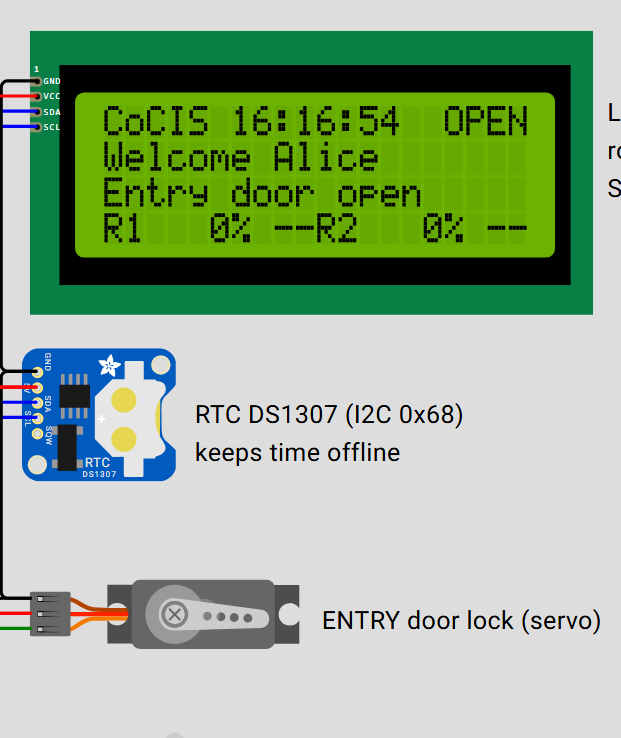
\includegraphics[width=\linewidth]{lcd-granted.png}\\[2pt]
  {\small (a) Granted: the entry door opens}
\end{minipage}\hspace{0.06\linewidth}
\begin{minipage}[b]{0.42\linewidth}
  \centering
  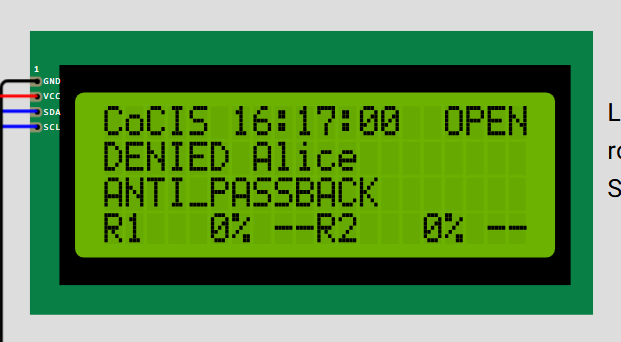
\includegraphics[width=\linewidth]{lcd-denied.png}\\[2pt]
  {\small (b) The same card again: anti-passback}
\end{minipage}
\caption{The LCD after card scans at the entry reader.}
\label{fig:lcd-scans}
\end{figure}

\consolefig{access}{Log records of four scans at the real readers: Alice enters, tries to enter
  again (anti-passback), leaves at the exit reader, then an unregistered key fob (captured in
  Wokwi).}

\paragraph{Leaving after hours.} The brief requires that people still inside after the access
period are not allowed to leave (\req{2.6}). We enforce this, and add two safety measures:
\begin{itemize}
  \item When an ordinary user is refused at the exit after hours, the hub logs
        \code{ALERT code=AFTER_HOURS_EXIT}, so security knows someone is waiting.
  \item When a \textbf{security} card exits after hours, an \textbf{escort window} opens for 60\,s,
        during which ordinary users may leave (\code{OK_ESCORT}). Security thus walks people out
        and every exit is still recorded.
  \item The \textbf{break-glass} button overrides every rule for life safety
        (\cref{sec:op-emergency}).
\end{itemize}

% ----------------------------------------------------------------------------
\subsection{Occupancy records (\req{2.1})}
The occupancy ledger (\file{services/occupancy.c}) is the list of cards currently inside. Only the
hub changes it, after a granted scan, and it is saved to NVS on every change, so a reboot does not
forget who is inside (the boot log prints \enquote{2 people inside at boot}). \code{who} prints the
list with entry times. This is the muster list for an evacuation. Together with the \code{ACCESS}
lines on the SD card, management can see who is inside now and who came and went at any time.

\consolefig{who}{\code{who} after Alice, Bob and Carol entered (captured in Wokwi).}

% ----------------------------------------------------------------------------
\subsection{Automatic lighting in the lecture rooms (\req{2.2})}
\label{sec:op-lighting}
Each room task (\file{nodes/room_node.c}) runs this loop every 200\,ms:
\begin{enumerate}
  \item Read any command from the hub (light mode AUTO, ON or OFF).
  \item Read the PIR (motion yes/no) and the LDR (light level in lux).
  \item Call the pure \code{room_logic_step()}, which decides occupancy, daylight and the lamp
        level.
  \item Move the lamp towards that level by 25\,\% per step, a soft 0.8\,s fade done in software.
  \item Report the new state to the hub when something changed (and every 60\,s), and send a
        heartbeat every 5\,s.
\end{enumerate}

\paragraph{The lighting rules} (\file{core_logic/room_logic.c}, AUTO mode):
\begin{itemize}
  \item \textbf{Occupancy.} Motion makes the room occupied. With no motion for the \emph{grace
        period} (30\,s) the room becomes vacant.
  \item \textbf{Pre-off warning.} During the last 10\,s of the grace period the lamp dims to
        30\,\%. Anyone still in the room moves and the light comes back to 100\,\%, instead of
        being plunged into darkness.
  \item \textbf{Daylight harvesting.} At or above 400\,lux the room counts as bright and the lamp
        stays off even if occupied. At or below 150\,lux it is dark again. Between the two, the
        last decision is kept (\emph{hysteresis}), so a cloud passing near one threshold does not
        make the light flicker.
  \item \textbf{Lamp level} is therefore 100\,\% if occupied and dark, 30\,\% during the warning,
        and 0\,\% if vacant or bright. ON and OFF (set by an admin with \code{light}) override it.
\end{itemize}

\paragraph{Energy accounting.} Each step adds the lamp's energy at its current level (360\,W
lamp bank per room, configurable) to \emph{energy used}. During opening hours it also adds full
power to a \emph{baseline}: what a room whose lights are simply left on all day would use.
\emph{Energy saved} = baseline $-$ used. The hub logs \code{ENERGY room=1 on_wh=... saved_wh=...}
for each room every 10\,minutes, and \code{rooms} shows the totals. This gives management a figure
for the electricity the system saves.

\consolefig{rooms}{\code{rooms} with daylight in Room~1 (650\,lux): vacant, lamp off, energy saved so far (captured in Wokwi).}

% ----------------------------------------------------------------------------
\subsection{Configurable access schedule (\req{2.6})}
\label{sec:op-schedule}
The schedule is an opening time, a closing time and the weekdays it applies to. The default is
07:00--22:00, Monday to Saturday. An admin changes it at any time:
\begin{lstlisting}[style=console]
cocis> schedule set 07:00 18:00 weekdays
\end{lstlisting}
If the closing time is earlier than the opening time, the window runs overnight (e.g.\
22:00--06:00, where the early-morning part belongs to the previous day's window). The new schedule
is validated, saved to NVS, takes effect immediately, and is logged as \code{CONFIG}. The LCD shows
the hours on row 2 and OPEN or SHUT on row 1. Changing the schedule requires an admin session, so
only authenticated personnel can do it (\cref{sec:op-auth}).

\consolefig{login}{Changing the schedule: refused without a session; \code{login}, the Red admin card at the exit reader, the PIN; then accepted and logged as \code{CONFIG} (captured in Wokwi).}

% ----------------------------------------------------------------------------
\subsection{Two-factor admin authentication (\req{2.6})}
\label{sec:op-auth}
Configuration commands need an admin session, which takes \textbf{two factors}: something you have
(the admin card) and something you know (a 4-digit PIN). The pure state machine
\file{core_logic/auth_fsm.c} drives it:

\begin{figure}[H]
\centering
\begin{tikzpicture}[node distance=8mm and 22mm]
  \node[state] (idle) {IDLE};
  \node[state,right=of idle] (card) {WAIT\_CARD};
  \node[state,right=of card] (pin) {WAIT\_PIN};
  \node[state,below=14mm of pin] (sess) {SESSION\\\footnotesize 5 min};
  \draw[arr] (idle) -- node[lbl,above]{\code{login}} (card);
  \draw[arr] (card) -- node[lbl,above]{admin card} (pin);
  \draw[arr] (pin) -- node[lbl,right]{correct PIN} (sess);
  \draw[arr] (card.south) to[out=-120,in=-60] node[lbl,below]{admin card refused / 30\,s timeout} (idle.south);
  \draw[arr] (pin.north) to[out=150,in=30] node[lbl,above]{wrong PIN / 30\,s timeout} (idle.north);
  \draw[arr] (sess.west) -| node[lbl,pos=0.25,below]{\code{logout} / session expires} (idle.south west);
\end{tikzpicture}
\caption{Admin login state machine. Three wrong PINs lock login for 60\,s.}
\label{fig:auth}
\end{figure}

\begin{enumerate}
  \item Type \code{login} on the serial console.
  \item Within 30\,s, present the admin card (Red) at either reader. The LCD shows
        \enquote{Admin login / PIN on console}. Any other card presented meanwhile is handled as a
        normal door request, so people keep coming and going during the login.
  \item Type \code{login 1234}. PINs are exactly 4 digits.
\end{enumerate}
PINs are never stored in clear text: the registry stores SHA-256 of a per-user random salt plus
the PIN. Every step (\code{CARD_OK}, \code{OK}, \code{BAD_PIN}, \code{LOCKED}, \code{TIMEOUT},
\code{LOGOUT}) is logged as an \code{AUTH} line, and a lockout also raises
\code{ALERT code=PIN_LOCKOUT}. The session ends after 5 minutes or on logout.

The console session in \cref{fig:con-login} shows the whole login.

% ----------------------------------------------------------------------------
\subsection{Data storage on the SD card (\req{2.4})}
\label{sec:op-storage}
Everything that happens becomes one text line on the SD card, in a new file every day:
\file{/sdcard/LOGS/YYYYMMDD.LOG}.
\begin{lstlisting}[style=console]
000010|2026-10-28T09:46:10|ACCESS|uid=01020304 name=Alice role=STUDENT side=IN ok=1 reason=OK|3f9a...c2
000014|2026-10-28T09:47:04|ROOM|room=1 occupied=0 daylight=0 lux=125|81d0...7e
\end{lstlisting}
The fields are: a sequence number, the local time, an event type, \code{key=value} details, and a
hash. The event types are \code{BOOT}, \code{ACCESS}, \code{ROOM}, \code{LIGHT}, \code{ENERGY},
\code{CONFIG}, \code{USER}, \code{AUTH} and \code{ALERT}; the full list of fields is in
\file{docs/event-schema.md}.

\paragraph{Tamper-evident hash chain.} The last field of each line is
$h_n = \mathrm{SHA\text{-}256}(h_{n-1} \,\|\, \texttt{"|"} \,\|\, \text{line}_n)$, with $h_0$ = 64
zeros at the start of each file. Changing, inserting or deleting any line changes every hash after
it. \code{log verify} recomputes the chain and reports the first broken line, so management can
trust that the records were not edited.

\paragraph{Reliability.} Only the storage task writes to the card. Each line is flushed and
\code{fsync}ed, so a power cut loses at most the line being written. After a reboot, the task reads
the last line to continue the sequence number and the chain. If the card is missing, logging
continues in a RAM ring buffer of the newest 32 lines and \code{ALERT code=SD_FAIL} is raised.
\code{log tail} shows recent lines either way.

\consolefig{log}{\code{log tail} and \code{log verify}: the newest records and the hash-chain check (captured in Wokwi).}

% ----------------------------------------------------------------------------
\subsection{Serial interface and management menus (\req{2.5})}
\label{sec:op-cli}
The serial console (\file{components/cli/}) gives a \code{cocis>} prompt with history and
\code{TAB} completion. \code{help} lists all commands; \cref{app:cli} gives the full reference.
The commands are grouped into monitoring (\code{status}, \code{who}, \code{rooms}, \code{users},
\code{log}), configuration for an admin (\code{schedule}, \code{user}, \code{light},
\code{lockdown}, \code{emergency}, \code{time}), the session (\code{login}, \code{logout}) and
simulation (\code{tap}, \code{node}).
With \code{log echo on}, every new log line is also printed live on the console as
\code{[LOG] ...}, which turns the terminal into a live event monitor.

% ----------------------------------------------------------------------------
\subsection{LCD, buzzer and LED}
\label{sec:op-ui}
A single \code{ui} task owns these outputs. Other tasks send it requests through a queue and never
wait for it. The 20$\times$4 LCD shows:
\begin{lstlisting}[style=console]
CoCIS 09:15:45  OPEN      <- clock and building state: OPEN, SHUT, LOCK or EMRG
Hours 07:00-22:00         <- or a 2-line message, e.g. "Welcome Alice / Entry door open"
Inside: 3      ADMIN      <- people in the building, admin session active
R1 100% P-R2   0% -S      <- per room: lamp %, P = people detected, S = enough sunlight
\end{lstlisting}
Only rows whose text changed are rewritten, so there is no flicker. The buzzer has distinct
patterns for granted, denied, information and alarm.

% ----------------------------------------------------------------------------
\subsection{Emergency, lockdown and node supervision}
\label{sec:op-emergency}
\begin{itemize}
  \item \textbf{Break-glass} (key \code{e}): both doors are held open, the alarm sounds, the LCD
        shows EMRG and \code{ALERT code=BREAK_GLASS} is logged. Only an admin can end it, with
        \code{emergency clear}.
  \item \textbf{Lockdown} (\code{lockdown on}): only security and admin cards pass, for example
        during an incident.
  \item \textbf{Node supervision.} Rooms send a heartbeat every 5\,s. If the hub hears nothing for
        15\,s it marks the room offline, shows \code{R2 offline} on the LCD and logs
        \code{ALERT code=NODE_OFFLINE}, and \code{NODE_ONLINE} when it returns. The room keeps
        controlling its own lights meanwhile.
\end{itemize}

\screenshot[0.3\linewidth]{lcd-emergency}{Break-glass emergency: both doors held open, EMRG on the LCD.}
  {Press e: LCD row 1 shows EMRG, both servos at 90 degrees.}
